% A Real Chapter
\chapter{Hyperbolic geometry and interest}

\section{Introduction to interest}
blabla

\section{Interest and hyperbolic functions}
The core motivation for the application of hyperbolic geometry on the problem of compound interest is the mathematical identity for hyperbolic functions
\begin{equation}
    \ininv e^{\han} = K\cosh(\han) + K\sinh(\han)
    \label{eq:sinhcosh}
\end{equation}
The left part in this equation is equal to the growth of money given a given period interest \han and subject to continuous compounding interest. For a constant interest rate over time $\han = \hanv t$:
\begin{equation}
    \ininv e^{\hanv t} = K\cosh(\hanv t) + K\sinh(\hanv t)
\end{equation}
where $\ininv$ equals the initial investement deposited. Using the hyperbolic functions, the growth of money can be visualised as traversing along a hyperbola in a plane, as visualised in [...], where $\hanv t$ is the so-called \textit{hyperbolic angle}. To define the latter, the notion of a \textit{hyperbolic sector} must be introduced first:

\begin{definition}[Hyperbolic sector]
    A hyperbolic sector is the region of the plane bounded by the rays from the origin to the points $(a, 1/a)$, $(b, 1/b)$, $a, b \in \real$. A hyperbolic sector in standard position has $a = 1$ and $b > 1$. 
    
\end{definition}

\begin{definition}[Hyperbolic angle]
    Consider the rectangular hyperbola $\{(x, 1/x)\ \vert\ x \in \real^+\}$. The hyperbolic angle in standard position is the angle at the origin between the ray $(1, 1)$ and the ray $(x, 1/x)$. The magnitude of this angle is equal to the area of the corresponding hyperbolic sector.
\end{definition}
These definitions are based on the \textit{rectangular hyperbola}, which is defined as the curve $xy = 1$. However, for the usage of hyperbolic functions and the further treatment in this chapter, the \textit{unit hyperbola} will be used as standard, which is described by $x^2 - y^2 = 1$. The only difference between the two is a \ang{45} rotation around the origin in either clockwise or counterclockwise. 

\begin{figure}
    \centering
    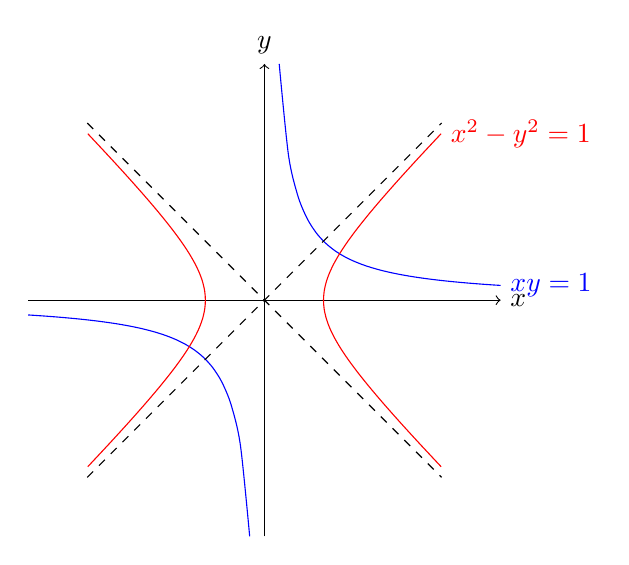
\begin{tikzpicture}[scale=1.5]
        \draw[->] (-2, 0) -- (2, 0) node[right] {$x$};
        \draw[->] (0, -2) -- (0, 2) node[above] {$y$};
        \draw[scale=0.5, domain=0.25:4, smooth, variable=\x, blue] plot ({\x}, {1/\x}) node[right] {$xy = 1$};
        \draw[scale=0.5, domain=-4:-0.25, smooth, variable=\x, blue] plot ({\x}, {1/\x});
        \draw[scale=0.5, domain=-1.76:1.76, smooth, variable=\x, red] plot ({cosh(\x)}, {sinh(\x)}) node[right] {$x^2 - y^2 = 1$};
        \draw[scale=0.5, domain=-1.76:1.76, smooth, variable=\x, red] plot ({-cosh(\x)}, {sinh(\x)});
        \draw[dashed] (-1.5, 1.5) -- (1.5, -1.5);
        \draw[dashed] (-1.5, -1.5) -- (1.5, 1.5);
    \end{tikzpicture}
    \caption{Comparison between rectangular hyperbola $(x, \tfrac{1}{x})$ (implicit equation $xy= 1$) and the unit hyperbola $(\cosh(t), \sinh(t))$ (implicit equation $x^2 - y^2 = 1$).}
\end{figure}

As such, a position vector of any point along the unit hyperbola can be decomposed along the rectangular axes using the hyperbolic functions in the same fashion as one would do for the unit circle with the `regular' trigonometric functions $\cos$ and $\sin$.

\begin{figure}
    \centering
    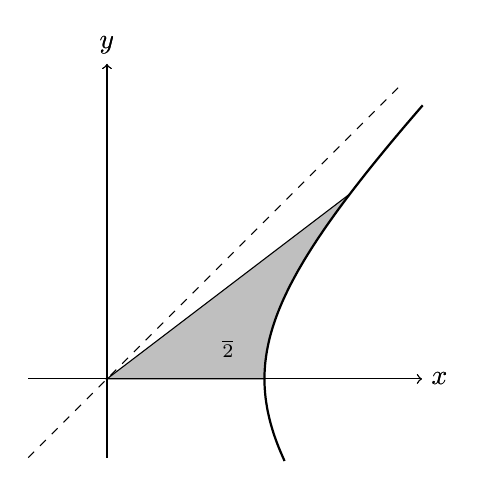
\begin{tikzpicture}[scale=2]
        \draw[->] (-0.5, 0) -- (2, 0) node[right] {$x$};
        \draw[->] (0, -0.5) -- (0, 2) node[above] {$y$};
        \filldraw[fill=gray!50] (0, 0) -- (1, 0) -- (1.54308, 1.1752) -- cycle;
        \filldraw[domain=-0.5:1.32, smooth, variable=\x, thick, fill=white] plot ({cosh(\x)}, {sinh(\x)});
        \draw[dashed] (-0.5, -0.5) -- (1.85, 1.85);
        \draw[->] (-0.5, 0) -- (2, 0) node[right] {$x$};
        \draw[->] (0, -0.5) -- (0, 2) node[above] {$y$};
        \draw (0.65, 0.2) node[right] {$\frac{\han}{2}$};
    \end{tikzpicture}
    \caption{Hyperbolic angle}
\end{figure}

If one considers a two-dimensional space where both axes have the units of money (\si{\money}), the accumulation of a unit sum of money as a result of compound interest over time is bound by the unit hyperbola, and the total amount of money outstanding is equal to the sum of the components of the abcissa and ordinate. Likewise, for an arbitrary initial sum \ininv the corresponding hyperbola is described by the equation $x^2 - y^2 = \ininv^2$. The resulting decomposition is given exactly by \cref{eq:sinhcosh}.

This finding giver rise to a first fundamental principle central to this dissertation:

\textit{
The accumulation of money as a result of compound interest is analogous to a hyperbolic rotational motion with constant hyperbolic angular velocity.}

The ultimate purpose of this concept is , as is customary in the field of economic engineering, to establish useful analogies between concepts from economics or finance and (mechanical) engineering. In this case an analogy can be made between finance/actuarial science and rotational mechanics, with the difference that one is concerned with hyperbolic motions as opposed to traditional circular or elliptic motions. Many parallels can be drawn between them --- this is the driving motivation for the relevance of the analogy --- but also have important discrepancies. These distinctions and theire ramifications on the `hyperbolic rotational mechanics' of finance are discussed in the upcoming sections.

\section{Hyperbolic geometry}
A deeper dive into the formalities of hyperbolic geometry.

\section{General interest accumulation}
The concept of compound interest is extremely old and well-understood and ubiquitous in modern-day finance. However, calculations are usually performed on a discrete basis, with monthly, semianual or annual compounding frequency. In the light mathematical elegance and a long-standing tradition in sytems theory, this problem will be approached using a continuous-time description (and compounding) first.

The exponential form of money accumulation $\amnt(t) = \ininv e^{\hanv t}$ no longer valid if further amounts are debited or credited at a later time, as would happen when loans are amortized or with line of credit (LOC) accounts. 

A second generalization must be made in the form of a varying interest. While many fixed-income assets feature a constant interest or perhaps a roll-over structure, there are also many situations where the governing interest rate is coupled to a benchmark interest such as the former LIBOR or current SOFR in Europe. [source?]

Taking these two generalizations into account, the following continuous-time differential equation (coined the general `interest equation') can be established to govern the growth of money under the most general circumstances:
\begin{equation}
    \dv{\amnt}{t} = \hanv(t) \amnt + u(t)
    \label{eq:interest_equation}
\end{equation}
where \hanv(t) represents the interest rate (or force of interest) and $u(t)$ the reduction or increase of the amount outstanding, for example by amortizations or additional withdrawals. 

\Cref{eq:interest_equation} is fairly reminiscent of standard LTI systems, only with \hanv(t) being time-dependent. Therefore, the case with constant interest rate will be addressed first, i.e. $\hanv(t) = \hanv \in \real \ \forall t$. The general solution of this equation is then
\begin{equation}
    \amnt(t) = A(0)e^{\hanv t} + \int_0^t e^{\hanv (t - \tau)} u(\tau )\dd{\tau}
\end{equation}
In general, the convolution term is hard to evaluate analytically for an arbitrary function $u(t)$. In contrast to general engineering applications, $u(t)$ will in finance virtually always have the form of discrete money transactions. These can be described by a sum of Dirac delta functions, i.e. 
\begin{equation}
    u(t) = \sum^N_{t=1} k_i \delta(t - t_i)
\end{equation}
with $k_i$ the transaction amount at time $t_i$ and $\delta(t)$ the classical Dirac delta function.

Since \cref{eq:interest_equation} is linear, one can consider the solution of just one discrete payment at a delayed moment in time and sum the corresponding solutions for each of the payments. Taking the Laplace transform of the corresponding expression yields

\begin{equation}
    \mathcal{L} 
    \qty{\dv{\amnt}{t} - \hanv(t) \amnt - k_i \delta(t - t_i)} = s\hat{\amnt}(s) - A(0) - \hanv\hat{\amnt}(s) - k_i e^{-t_i s}
\end{equation}

\section{Hyperbolic kinematics}
\subsection{Hyperbolic coordinates}

\section{Angular momentum}

\section{Kinetic energy}

\section{Potential energy}
Explore the idea of a potential field capturing the need for people to
